\chapter{Coding and layout construction}\label{ch:coding-and-layout-construction}

This chapter is the central part of the thesis
as it presents the novel genetic approach, which is demonstrated in solving the painting placement problem.
In section~\ref{sec:genetics}, definitions regarding genetics are laid out together with the Schema Theorem description.
Section~\ref{sec:coding} describing individual representation and section~\ref{sec:operators}
describing genetic operators together present the novel genetic approach.
Section~\ref{sec:layout-construction} describes a greedy placing heuristic
used to construct the painting placement layout.
Lastly, section~\ref{sec:reproductive-plan} describes the reproductive plan.

\section{Genetics}\label{sec:genetics}

This section describes critical genetic terms that are used throughout the thesis.
They are allele, gene, chromosome, individual, population, crossover, mutation, and reproductive plan.
Also, in subsection~\ref{subsec:schema-theorem}, the integral part of genetics called the Schema Theorem is described.

First, it is essential to describe what the genetic approach means.
The genetic approach was first introduced by Holland in 1975
to solve optimization problems where it is computationally infeasible to
find an optimal solution by enumerating all possible solutions~\cite{hollandAdaptationNaturalArtificial1975}.

This genetic approach is inspired by nature and Darwin’s Theory of Evolution
– a population of individuals evolving over time.
Individuals more adapted to the environment are
more likely to survive and thus pass their genes to the next generation.
Thus, over time, the population should converge to the state where the adaptation to the environment is the highest~\cite{darwinOriginSpeciesMeans2009}.

Holland in~\cite{hollandAdaptationNaturalArtificial1975} defines several structures that reassemble this natural process.
The most important ones are described in the rest of this section.\\

\navesti{Allele} represents a concrete value that a gene can have.
It can be thus described as a set of alternatives to choose from. \\

\navesti{Gene} is a structure composed of alleles.
It often describes one trait or characteristic. \\

\navesti{Chromosome} is a structure composed of genes.
Thus it is an amalgam of characteristics described by genes.\\

\navesti{Individual} is defined by its chromosome and represents a solution to the problem or a structure from which a solution can be constructed.
A numeric value called \definice{fitness} can be assigned to each individual, representing how well the individual performs in an environment. \\

\navesti{Population} is a set of individuals.
It can be interpreted as a subset of possible solutions.\\

One concrete example of the abovementioned definitions is in figure~\ref{fig:population}.
There are two individuals in the population, with their chromosomes having two genes.
The first gene is a vector containing permutation with alleles of 1 to 5.
The second gene is a string vector
with alleles having values $H$ or $V$.
Lastly, each individual has a fitness value.
Thus, because A’s fitness $30.5$ is greater than B’s fitness $9.8$, we can say that individual A performs better than B.


\begin{figure}
    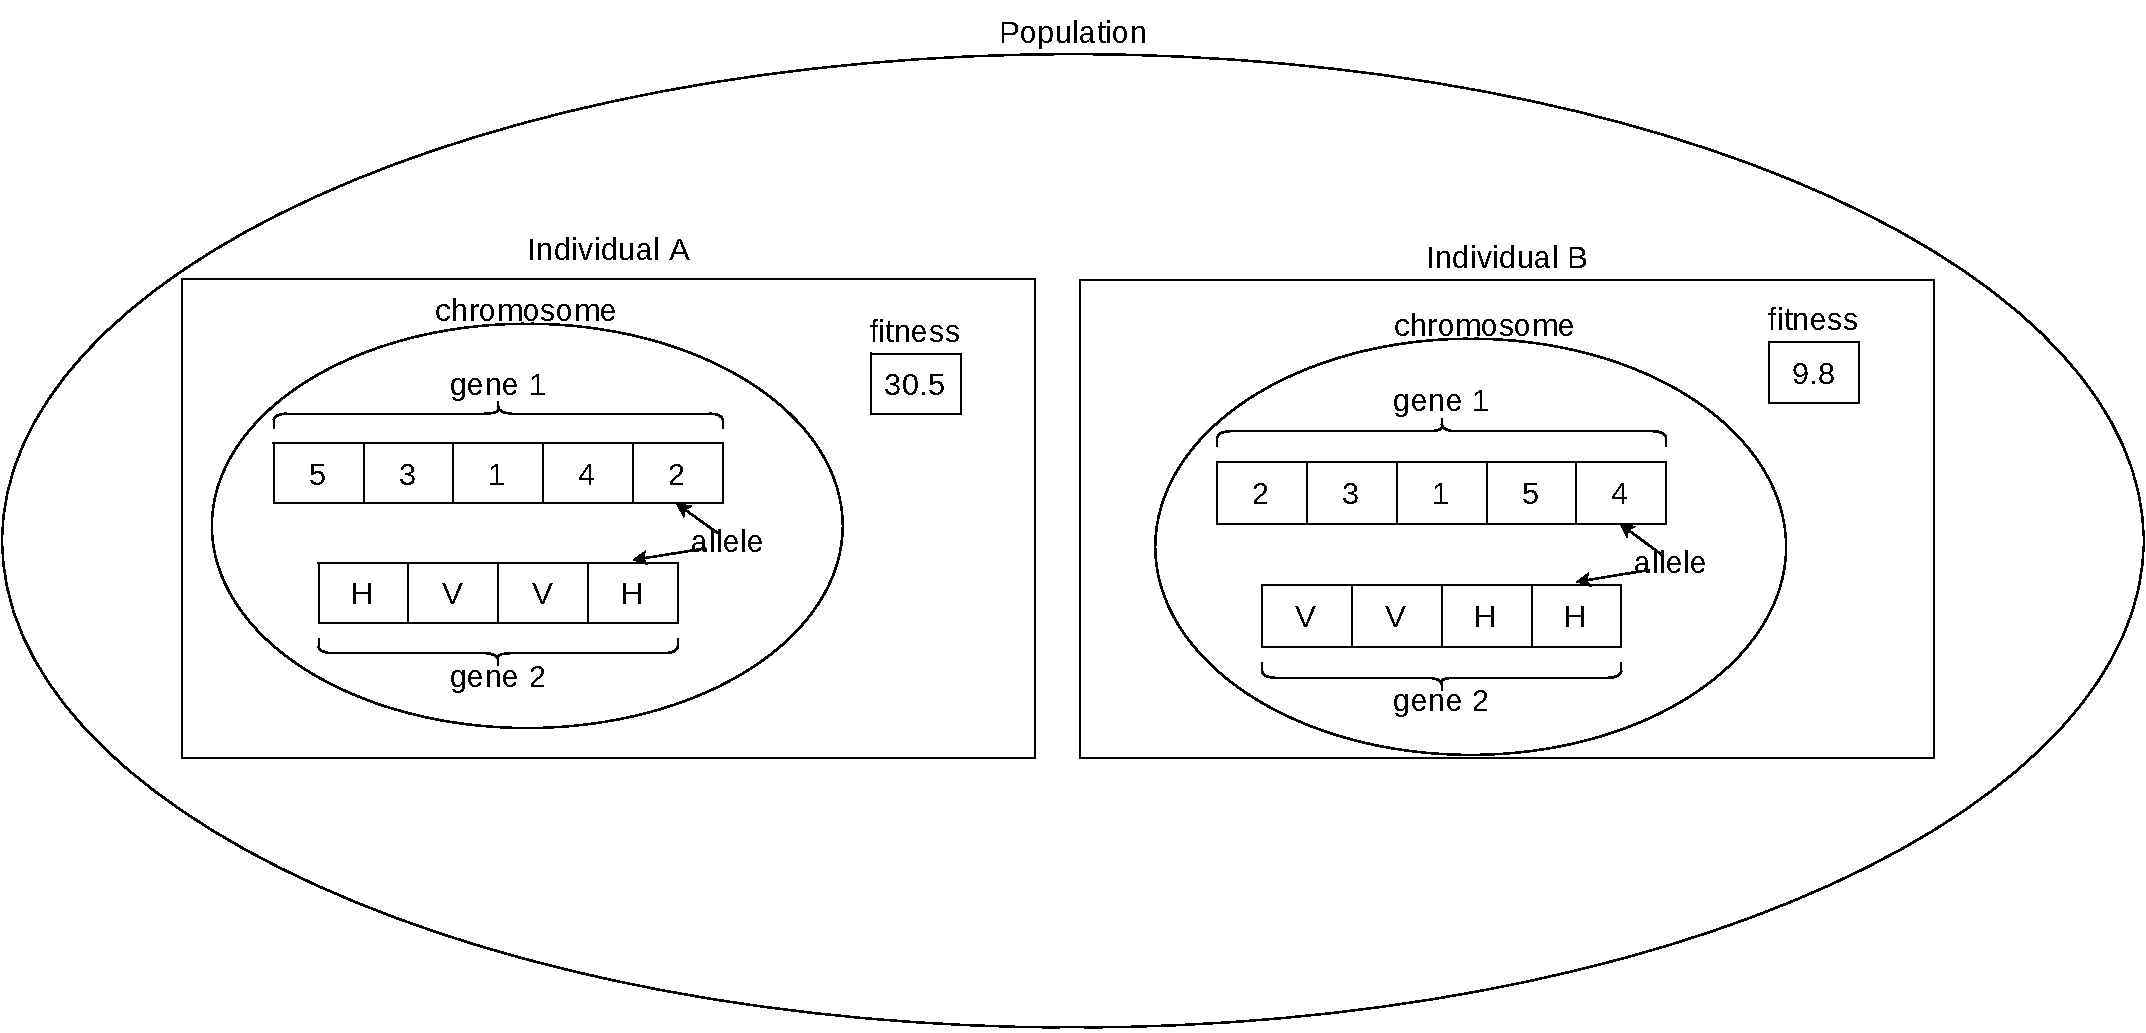
\includegraphics[width=1.1\textwidth, left]{population}
    \caption[Population example]{Example of a population composed of two individuals.}
    \label{fig:population}
\end{figure}

For the structures defined above, multiple operations called \definice{genetic operators} or simply operators
are defined by Holland and used by other researchers following his work.
Genetic operators aim to create new individual/s using individuals already present in a population as input.
Two of them that are used in this thesis are described below.\\


\navesti{Crossover} genetic operator takes two individuals as input and, by recombination
of their alleles in their genes, produces a new individual/s called \definice{offspring} or \definice{child}.\\

\navesti{Mutation} genetic operator takes one individual as input and produces a new one
which may have some of its alleles replaced by different ones at random.\\

Finally, there needs to be a process that transforms a population
to a new one with the goal of if this transformation process is applied sufficient
number of times to some initial population,
(sub)-optimal solution to the problem will be found.
This process is called the reproductive plan.\\

\navesti{Reproductive plan} is a process that takes a population on input and produces a modified
population using genetic operators.\\

One example of a reproductive plan is in figure~\ref{fig:reproductive-plan}.
At the start, an initial population of individuals is generated.
Then, for each individual, the fitness value is calculated.
Lastly, two genetic operators are applied to produce the new population.
In this example, crossover and mutation.
The process ends if the stopping condition is met.

\begin{figure}[h]
    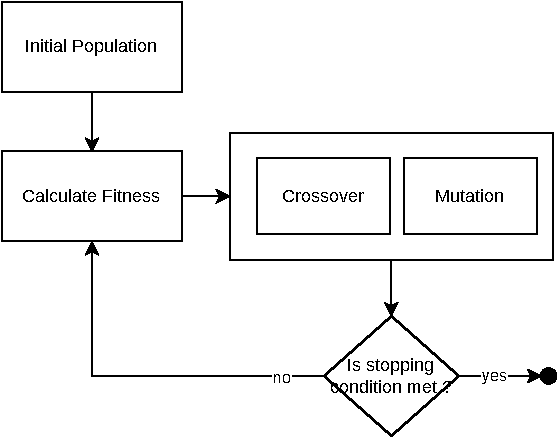
\includegraphics[width=0.65\textheight, center]{reproductive_plan}
    \caption[Example of a reproductive plan]{Example of a reproductive plan with crossover and mutation genetic operators.}
    \label{fig:reproductive-plan}
\end{figure}

\subsection{Schema Theorem}\label{subsec:schema-theorem}

Holland in~\cite{hollandAdaptationNaturalArtificial1975} proposed
the Schema Theorem arguing why the genetic approach described above works.
This subsection describes the main idea behind the argument.
First, an important term to describe is the schema.\\

\navesti{Schema} is an extended representation of chromosome,
where each gene can contain a “don’t care” symbol marked as underscore $\_$.
This symbol can take up any value that an allele can in the given context.
We can then say that chromosome belongs to a schema
and that schema contains a chromosome.\\

Schema can be illustrated on a chromosome with one gene represented as a vector that contains a permutation of numbers $1$ to $7$.
Then, example of a schema is $H_1 = \langle 5, \_, \_, 2, \_, 3, \_ \rangle$.
It contains $24$ chromosomes, with one example being $\langle 5, 4, 1, 2, 6, 3, 7 \rangle$.
On the other hand, schema $H_2 = \langle 1, 2, 3, 4, 5, 6, \_ \rangle$ contains only one chromosome.

There are two other properties that a schema has. They are length and order and are defined as follows.\\

\definice{Length} of a schema is the distance from the first “non-don’t care” symbol to the last.\\

\definice{Order} of a schema is the number of “non-don’t care” symbols contained in the schema.\\

For example, $H_1$ has length $6$ and order $3$.
It is graphically illustrated in figure~\ref{fig:schema}.
On the other hand, schema $H_2$ has the same length, $6$, but higher order, which is also $6$.

With schema being defined, we can interpret any population of individuals as a pool of schemata.
It can then be reformulated that a genetic approach, which has a reproductive plan and
genetic operators, (1) creates new schemata by recombination of the one already present in the population,
(2) creates schemata that are absent in the population, and (3) keeps a history of the best schemata found.
The Schema Theorem can then be written as

\begin{equation}
    \mathrm{E}[M(H, t+1)] \geq M(H, t) \dfrac{\mu(H)}{\overline{\mu}}\left[ 1 - p_c \dfrac{\delta(H)}{k-1} - \sigma(H)
    p_m \right]\,,
    \label{eq:schema-theorem}
\end{equation}

where $M(H, t)$ is expected number of individuals whose chromosome belongs to schema $H$ in population $t$,
$\mu(H)$ is average fitness of individuals whose chromosome belongs to $H$,
$\overline{\mu}$ is average population fitness,
$\delta(H)$ is length of schema $H$ with it’s maximum length $k$,
$\sigma(H)$ is order of $H$,
$p_c$ is crossover probability, and
$p_m \ll 1$ is mutation probability.

Inequality~\ref{eq:schema-theorem} says, that the success of a schema $H$,
considering only crossover and low probability mutation are purely determined
by its better-than-average performance, length, and order.
It can be thus said that the genetic approach favors
short schemata with low order that have better-than-average performance.

The reasoning behind the argument is that schemata with high order are more likely
to be damaged by mutation, i.e., an allele of a schema is replaced by a different one.
Also, longer schemata are more likely to be split using a crossover, whereas Holland
considers a one-point-crossover that produces an offspring’s chromosome by copying
of the first parent’s chromosome up to the crossover point, followed by the second parent chromosome after the crossover point.

\begin{figure}[h]
    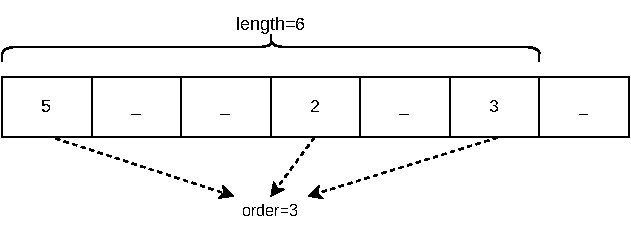
\includegraphics[width=0.7\textwidth, center]{schema}
    \caption[Example of a schema]{Example of a schema, where “don’t care” symbol marked as underscore $\_$.}
    \label{fig:schema}
\end{figure}

\section{Coding}\label{sec:coding}

The central part of the novel genetic approach proposed in this thesis is how an individual is represented.
This is important not only for the construction of the genetic operators, e.g., crossover and mutation
but also for the process of decoding an individual from its representation to the solution.

An individual is represented as a 3D chromosome—which means having three genes—that is composed of
(1) painting sequence random key, (2) slicing order random key, and (3) orientation probabilities.
An example of a chromosome is in figure~\ref{fig:chromosome}.

Let us use the notation for painting sequence random key as $PS_{rk}$,
slicing order random key as $SO_{rk}$,
orientation probabilities as $OR_{prob}$ and instance size as $N$, i.e., number of paintings.
First two are vectors, where $PS_{rk} \in \real^N$ and $SO_{rk} \in \real^{N-1}$.
Orientation probabilities is a matrix where $OR_{prob} \in \real^{N-1, 3}$.
Constraints in~\ref{eq:constraints} apply to each of these parts with
a stochastic vector meaning a vector that contains non-negative elements that add up to one.

\begin{equation}
    \begin{aligned}
        & 1. \quad PS_{rk} \text{ is a stochastic vector.} \\
        & 2. \quad SO_{rk} \text{ is a stochastic vector.} \\
        & 3. \quad \text{Each row in } OR_{prob} \text{ is a stochastic vector.}
    \end{aligned}\label{eq:constraints}
\end{equation}


The above-mentioned representation is based on a solution to the FLP
from~\cite{friedrichIntegratedSlicingTree2018, riponAdaptiveVariableNeighborhood2013},
where the authors represent an individual as a 3D chromosome with concrete identifiers for facilities, slicing order, and orientations.
However, the novel approach to coding proposed in this thesis are (1) the use of the stochastic vectors, (2) the use of random keys, (4) novel mutation and crossover operator, and
(3) introduction of novel decoding of an individual.
Thus, the search in the proposed genetic approach takes place in a different space, which is a space of stochastic vectors.

\begin{figure}[htp]
    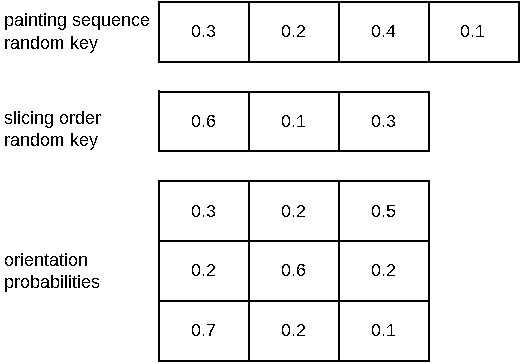
\includegraphics[width=0.8\textwidth, center]{chromosome}\caption[Example of an individual representation]{
        Example of an individual representation – two vectors and one matrix.
        Each vector and matrix row form a stochastic vector, i.e., they contain non-negative elements that add up to one.
    }
    \label{fig:chromosome}
\end{figure}

There are multiple ideas behind representing an individual as a set of stochastic vectors that stem
from extending RKGA~\cite{beanGeneticAlgorithmsRandom1994}, where chromosome is represented as a vector of values from $\langle0,1\rangle$.
First of them is the ability to perform mutation at an arbitrary element of these vectors using
a simple replacement, i.e., substituting an element for a random one from interval $\langle0,1 \rangle$,
followed by normalization back to the stochastic vector.
For example, using representation described in~\cite{friedrichIntegratedSlicingTree2018, riponAdaptiveVariableNeighborhood2013},
there has to be a different mutation method for each part of a chromosome.
By using the representation proposed in this thesis, there has to be only one mutation operator that can be used universally for all parts of the chromosome.

Additionally, when using representations similar to~\cite{friedrichIntegratedSlicingTree2018, riponAdaptiveVariableNeighborhood2013},
after the application of the genetic operators, usually crossover and mutation, an invalid individual might be created.
That is an individual that does not represent any solution.
The presence of invalid individuals might lead to performance loss in FLP~\cite{liuMultiimprovedGeneticAlgorithm2012}.
Moreover, unique solutions for dealing with invalid individuals must be introduced.
For example, left-to-right scan used by~\cite{hwangGeneticAlgorithmApproach2009, kandasamyEffectiveLocationMicro2020}
or leaving invalid individuals inside the population but penalizing them~\cite{hwangGeneticAlgorithmApproach2009}.
The solution proposed in this thesis produces only valid individuals.

Finally, the reasoning behind using a stochastic vector as opposed to a vector from $\langle0,1\rangle$ in RKGA~\cite{beanGeneticAlgorithmsRandom1994}
is the unique implementation of crossover used in this thesis, which is described in subsection~\ref{subsec:crossover}.

\newpage
\section{Solution construction}\label{sec:solution-construction}

This section describes the process of how to transform or decode an individual.
This transformation aims to create a solution to the painting placement problem,
which is a sequence of placement points for the paintings.
There are multiple steps to this process.

\begin{enumerate}
    \item Individual decoding (\ref{subsec:individual-decoding}).
    \item Slicing tree construction (\ref{subsec:slicing-tree-construction}).
    \item Slicing layout construction (\ref{subsec:slicing-tree-construction}).
    \item Using placement heuristic to create a painting placement solution (\ref{subsec:placement-heuristic}).
\end{enumerate}

Steps in the transformation of an individual to the painting placement solution are
in figure~\ref{fig:layout-construction-steps}.
All of these steps are explained in the following text.


\begin{figure}[h!]
    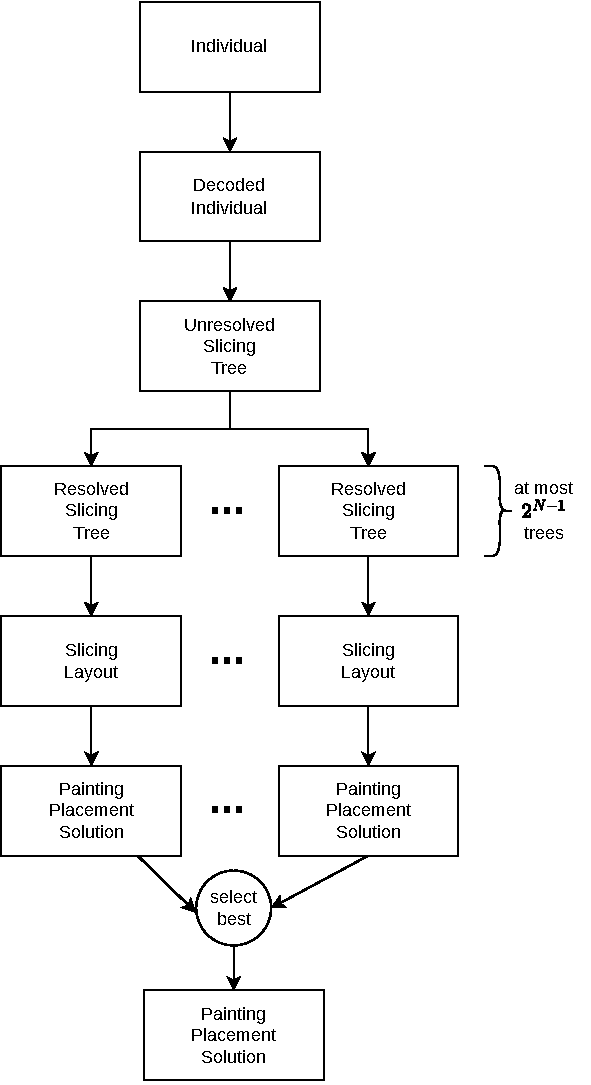
\includegraphics[height=0.65\textheight, center]{layout_construction_steps}
    \caption[Transformation of an individual to the painting placement solution]
    {Steps in the transformation of an individual to the painting placement solution.}
    \label{fig:layout-construction-steps}
\end{figure}

\subsection{Individual decoding}\label{subsec:individual-decoding}
First, we must decode an individual to the representation from which a slicing layout can be constructed.
A decoded individual is composed of painting sequence, slicing order, and orientations.
An example of individual decoding is in figure~\ref{fig:individual-decoding}.

Let us use the notation for painting sequence as $PS$, slicing order as $SO$, and orientations as $OR$.
$PS$ contains painting identifiers, $SO$ contains information used to construct slicing layout,
and $OR$ contains type of the cuts.\\

\navesti{Cut type} in $OR$  can take up three values.
\begin{itemize}
    \item $H$ for horizontal.
    \item $V$ for vertical.
    \item $*$ for wildcard, that can take up any value $H$ or $V$.
\end{itemize}

The introduction of the wildcard cut type $*$ is a novel idea proposed in this thesis.
In literature, only $H$ and $V$ cut types are used~\cite{friedrichIntegratedSlicingTree2018, changSlicingTreeRepresentation2013, liuMultiimprovedGeneticAlgorithm2012, hwangGeneticAlgorithmApproach2009}.

\subsubsection*{Decoding random keys}

Decoding $PS_{rk}$ to $PS$ and $SO_{rk}$ to $SO$ is the same as the RKGA in~\cite{beanGeneticAlgorithmsRandom1994}.
The graphical illustration is in figure~\ref{fig:individual-decoding} marked as~\textit{random key decoder}.
Decoding random keys in $PS_{rk}$ and  $SO_{rk}$ can be explained in the following steps on a sequence of four numbers $S = 0.3, 0.2, 0.4, 0.1$\,.

\begin{enumerate}
    \item Create $S'$ by adding a lower index to each element from $S$, which marks its ordinal position starting from one.
    $S' = 0.3_1, 0.2_2, 0.4_3, 0.1_4$\,.
    \item Sort $S'$ in descending order. $S' = 0.1_4, 0.2_2,  0.3_1, 0.4_3$\,.
    \item Take lower indexes of $S'$.
    It is the result – $4, 2, 1, 3$.
\end{enumerate}


\subsubsection*{Orientation probabilities decoding}

Last part of the individual, matrix $OR_{prob} \in \real^{N-1, 3}$, decodes to $OR$, which is a sequence of cut types.
The graphical illustration is in figure~\ref{fig:individual-decoding} marked as~\textit{orientation decoder}.

Decoding $OR_{prob}$ to $OR$ translates each row to one cut type.
Thus, decoding orientation probabilities can be explained for one row, say $R = 0.7, 0.2, 0.1$
in the following steps.


\begin{enumerate}
    \item Create $R'$ by adding lower index $H$ to the first, $V$ to the second, and $*$ to the last $R$'s elements.
    $R' = 0.7_H, 0.2_V, 0.1_*$
    \item Select element from $R'$ with the maximum value. $\max R' = 0.7_H$.
    \item Take lower index of $\max R'$.
    It is the result – $H$.
\end{enumerate}

There is one exception to the steps described above.
It is the limit on the maximum number of $*$ cut types produced by $OR_{prob}$ decoding.
Let us call this limit $k$.
If the limit is not applicable, i.e., $k \geq N-1$, there is no change to decoding steps 1--3 described above.
However, only the first $k$ wildcard cut types $*$ with the highest value are considered if applicable.
It is achieved by setting the value to $0$ (only for the duration of the decoding) to the bottom $N-1-k$ wildcard cut types $*$ with the lowest values.
Then the same 1--3 decoding steps are applied as described above.

One example where the limit on wildcard cut types $*$ applies is for the $k=1$ and $OR_{prob}$ that has two rows, $R_1 = 0.2, 0.3, 0.5$ and $R_2 = 0.1, 0.2, 0.7$.
Without exception, the result is $*, *$.
However, considering the exception on the maximum limit $k=1$, the result is $V, *$.
Reason is that in $R_2$, wildcard $*$ has value $0.7$,
which is higher than value of $*$ in $R_1$, which is $0.5$.

\begin{figure}[h!]
    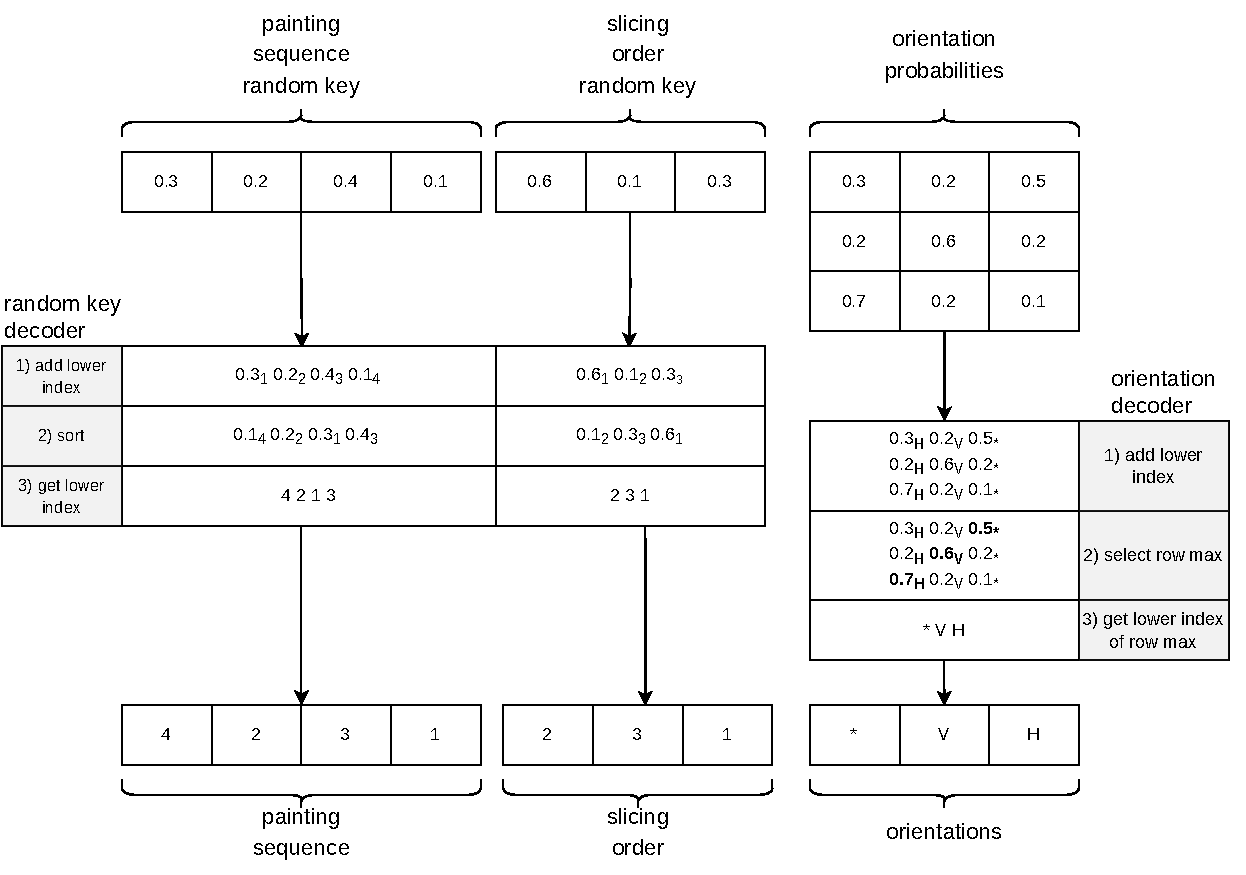
\includegraphics[width=1.1\textwidth, left]{individual_decoding}
    \caption[Individual decoding example]{
        Individual decoding example. Both the painting sequence random key and slicing order random key
        are decoded using the same procedure.
        The decoded individual is used to construct an unresolved slicing tree. }
    \label{fig:individual-decoding}
\end{figure}

\subsection{Slicing layout construction}\label{subsec:slicing-tree-construction}
In the previous subsection, decoding an individual is described.
The decoded individual consists of three parts – painting sequence, slicing order, and orientations.
From this representation, a slicing layout can be constructed.\\

\navesti{Slicing layout} is the recursive partitioning of space to rectangles using horizontal and vertical cuts.\\

Construction of the slicing layout from painting sequence, slicing order, and orientations has three steps, which are as follows.

\begin{enumerate}
    \item Construct an unresolved slicing tree from a decoded individual.
    \item Resolve an unresolved slicing tree.
    \item Create a slicing layout using a resolved slicing tree.
\end{enumerate}

\subsubsection*{Slicing tree construction}

First, let us describe what a slicing tree is.
The slicing tree was first introduced in 1982 by Otten~\cite{ottenAutomaticFloorplanDesign1982} to solve automatic floorplan design.
In the most general sense, it is a tree that codes the recursive division of space into rectangles using horizontal and vertical cuts.
A slicing tree can thus be used to construct a slicing layout.
According to~\cite{laiSlicingTreeComplete2001}, a slicing tree is a complete representation of a slicing layout.
That means that every possible slicing layout has at least one slicing tree that represents it.
This thesis defines and uses the slicing tree in two variants.\\

\navesti{Resolved slicing tree} is a binary tree with internal nodes having values from $\{H, V\}$
and leafs having values from the painting sequence.\\

\navesti{Unresolved slicing tree} is an extension of a resolved slicing tree where internal nodes have values from $\{H, V, *\}$. \\

Cut types $H$ for horizontal and $V$ for vertical are common for both types of the slicing tree.
An unresolved slicing tree can also contain the wildcard cut type $*$.

Next, we can use a decoded individual to construct an unresolved slicing tree.
This construction is graphically illustrated in the left part of a figure~\ref{fig:slicing-tree-construction}.
During this process, the painting sequence results in leaf nodes, slicing order determines the shape of a tree, and orientations are the values assigned to internal nodes.
Thus, each decoded individual represents one unresolved slicing tree.

Finally, an unresolved slicing tree is resolved.
Resolving is graphically illustrated in the right part of a figure~\ref{fig:slicing-tree-construction},
where the unresolved tree contains one wildcard symbol $*$ as a root.
By resolving this tree, $*$ is first replaced by $H$ and then by $V$.
In this case, resolving the unresolved slicing tree produces two resolved slicing trees,
which differ in root node value.
In the general case, an unresolved slicing tree can at most resolve to $2^k$ resolved slicing trees,
where $k$ is the number of internal nodes, i.e., the nodes that can contain wildcard $*$.
Reformulation for a decoded individual is that decoded individual can, at most, represent
$2^k$ resolved slicing trees, where $k$ is the number of orientations.



\subsubsection*{Slicing layout}

Next, we can construct a slicing layout using a resolved slicing tree.
Input to the construction has three parts that are as follows.

\begin{enumerate}
    \item Layout to partition.
    \item Areas of paintings to place.
    \item Resolved slicing tree
\end{enumerate}

The layout is the wall on which the paintings are placed.
Areas of the paintings are retrieved using the resolved slicing tree,
which contains painting identifiers as leaf nodes.

Construction can be described using figure~\ref{fig:slicing-layout-dimensions}.
On the left is an input to the construction – three paintings $1,2,3$ with areas $a_1, a_2, a_3$ and resolved slicing tree.
Then, we recursively traverse the resolved slicing tree.
Depending on the node value, there are three possible actions. \todo{mozna dodat pseudokod?}

\begin{itemize}
    \item $H$ – cut layout horizontally.
    \item $V$ – cut layout vertically.
    \item Otherwise, assign node value to the layout.
\end{itemize}

After performing the cut, the process mentioned above is recursively repeated
for the left and right child.
If the cut is horizontal, the left child is given the upper part of the cut as its layout, and the right child is given the lower part.
If the cut is vertical, the left child is given the left part of the cut as its layout, and the right child is given the right part.
It can be seen in the middle part of the figure, where the cut is vertical.
The left child is an orphan, i.e., it has no children.
Thus, the left part of the cut is assigned value 1.
The right child is not an orphan, meaning the process is applied recursively to the right part of the cut and the right child.
It is depicted on the right part of the figure.

The last part of creating a slicing layout is the position of the cut.
As mentioned above, there are horizontal and vertical cut types at the resolved slicing tree.
Each cut type's position is determined proportionally to the area of rectangles assigned to the cut result.
Again, it can be described using an example in figure~\ref{fig:slicing-layout-dimensions}.
The first cut is vertical, where the left part of the cut is assigned rectangles $1$ and the right part is assigned rectangles $2,3$.
The vertical cut thus splits the layout into two parts – the left part having $1/3$ of the total layout area and the right part
having the rest.

\afterpage{%
    \clearpage% Flush earlier floats (otherwise order might not be correct)
    \begin{landscape}% Landscape page
        \begin{figure}[]
            \centering
            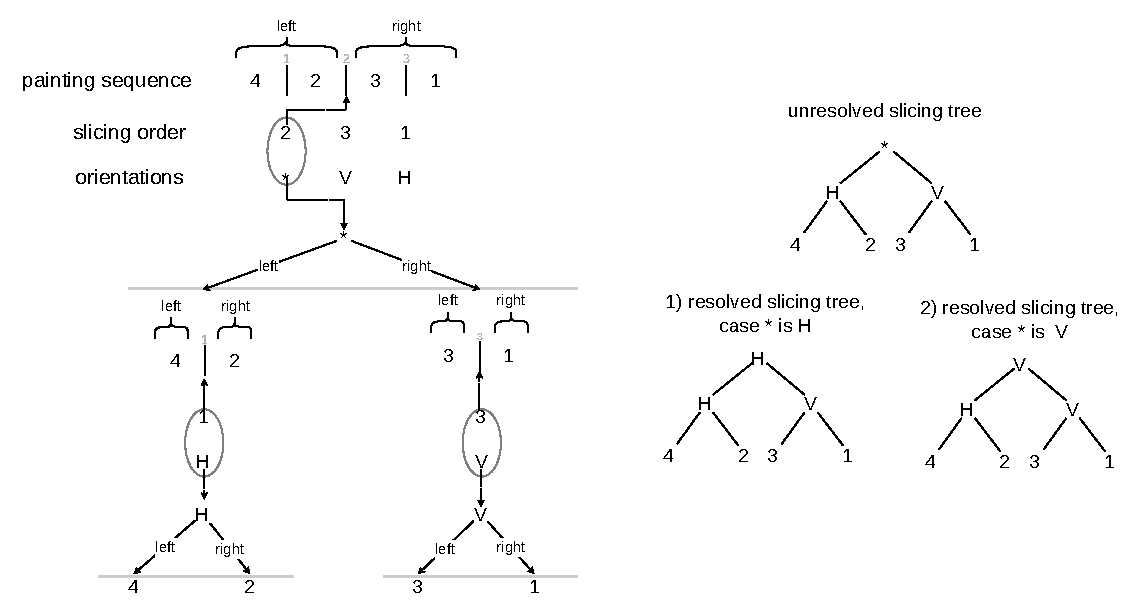
\includegraphics[width=1.5\textwidth]{slicing_tree_construction}
            \caption[Slicing tree construction]{
                On the left is an example of unresolved slicing tree construction from a decoded individual.
                On the right is an example of resolving an unresolved slicing tree.}
            \label{fig:slicing-tree-construction}
        \end{figure}
    \end{landscape}
    \clearpage% Flush page
}

\afterpage{%
    \clearpage% Flush earlier floats (otherwise order might not be correct)
    \begin{landscape}% Landscape page
        \begin{figure}
            \centering
            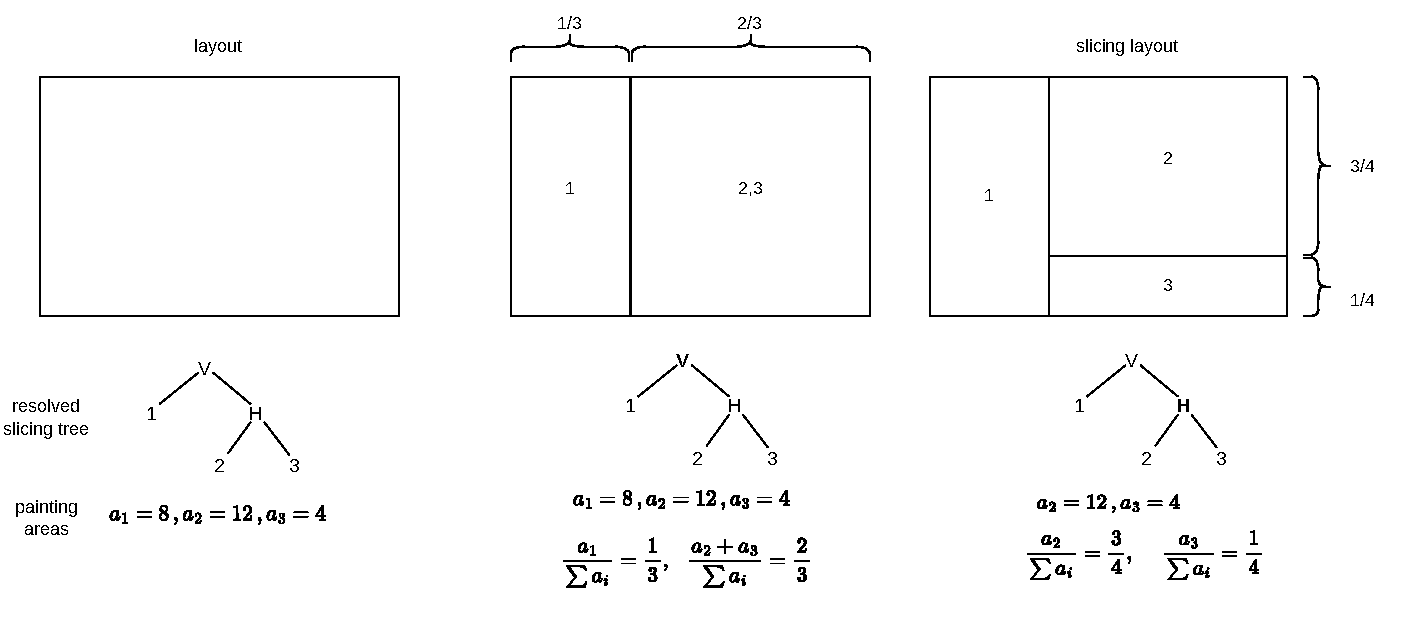
\includegraphics[width=1.5\textwidth]{slicing_layout_dimensions}
            \caption[Slicing layout construction]
            {Example of a slicing layout construction from a resolved slicing tree, painting areas and layout. There are three paintings, $1,2,3$ together with their areas $a_1, a_2, a_3$.
            The position of a cut is determined proportionally to the area of the paintings.} \label{fig:slicing-layout-dimensions}
        \end{figure}
    \end{landscape}
    \clearpage% Flush page
}


\newpage

\subsection{Placement heuristic}\label{subsec:placement-heuristic}

The placement heuristic is the last part of transforming an individual into a painting placement solution.
Input to the heuristic is the slicing layout together with paintings, and output is the painting placement solution.
The pseudocode of the proposed placing heuristic is in algorithm~\ref{alg:placement-heurictic}

\begin{algorithm}[H]
    \SetAlgoLined
    \LinesNumbered

    \SetKwData{PlacedPaintings}{placedPaintings}
    \SetKwData{Painting}{painting}
    \SetKwData{PlacedPainting}{placedPainting}
    \SetKwData{Paintings}{paintings}
    \SetKwData{Best}{best}
    \SetKwData{SlicingLayout}{slicing layout}
    \SetKwData{Nil}{NIL}
    \SetKwData{EmptyList}{EMPTY LIST}

    \SetKwFunction{PossiblePlacementPoints}{possiblePlacementPoints}
    \SetKwFunction{Place}{place}
    \SetKwFunction{Objective}{objective}

    \SetKw{In}{in}
    \SetKw{Or}{or}


    \KwData{\SlicingLayout, \Paintings}
    \KwResult{painting placement solution} \BlankLine

    %%%%%%%%%%%%%%%%%%%%%%%%

    \PlacedPaintings $\leftarrow$ \EmptyList \\

    \For{$painting$ \In \Paintings} {
        \Best $\leftarrow$ \Nil \\
        \For{$point$ \In \PossiblePlacementPoints{painting, \PlacedPaintings, \SlicingLayout}} {
            \PlacedPainting $\leftarrow$ \Place{painting, point}\\
            \If{\Best == \Nil \Or \Objective{\PlacedPainting} <  \Objective{\Best}}{
                \Best $\leftarrow$ \PlacedPainting
            }
        }
        \PlacedPaintings += \Best
    }

    \KwRet{\PlacedPaintings}

    \caption{Placement heuristic}\label{alg:placement-heurictic}
\end{algorithm}

The proposed heuristic is greedy and iterative.
Iterative means that it creates the painting placement solution gradually, as it
tries to place one painting after another using the slicing layout.
It is greedy because, at each iterative step, it places a painting in a way that minimizes the objective value.

An important part of the heuristic placement algorithm~\ref{alg:placement-heurictic}
is function \verb|possiblePlacementPoints| on line 4.
This function returns points that the heuristic tries for placing a painting.
Furthermore, it is the only part that uses a slicing layout.

As mentioned earlier, the slicing layout divides space into rectangles.
Additionally, each rectangle in the slicing layout has been assigned a painting.
The function \verb|possiblePlacementPoints| uses this assigned space as allocated area.\\

\navesti{Allocated area} for a painting is a rectangle from a slicing layout to which it was assigned.\\

This means that every slicing layout has one allocated area for each painting.
Also, the allocated area does not necessarily need larger dimensions than the painting.
E.g., the width of a painting might be greater than the width of its allocated area.
An example of a painting and its allocated area is in figure~\ref{fig:allocated-area}.

With the defined allocated area,
we can describe which implementation is used for the function \verb|possiblePlacementPoints|.
It is called the corner-placing heuristic.\\

\navesti{Corner-placing heuristic} is a placing heuristic that considers four painting placement points for each painting
– the allocated area's bottom-left, bottom-right, top-left, and top-right corners.\\

Examples of the painting placement points created by the corner-placing heuristic are in figure~\ref{fig:allocated-area}.
On the left, we can see that the allocated area's dimensions are sufficient
to try all four points.
In the middle, there are only two points where the placing of a painting does not
result in it being outside the allocated area.
On the right, all points result in being outside the allocated area.
Additionally, figure~\ref {fig:corner-placing-heuristic} shows iteration of the corner-placing heuristic considering one placement point.

\begin{figure}[h!]
    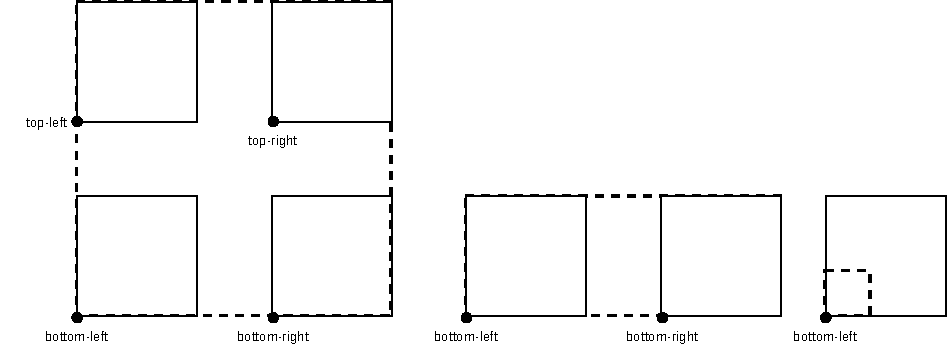
\includegraphics[width=1.2\textwidth, center]{allocated_area}
    \caption[Examples of the painting placement points created by the corner-placing heuristic]
    {Examples of the painting placement points created by the corner-placing heuristic
    for three different allocated areas that are plotted using a dashed line.}
    \label{fig:allocated-area}
\end{figure}

\begin{figure}[h!]
    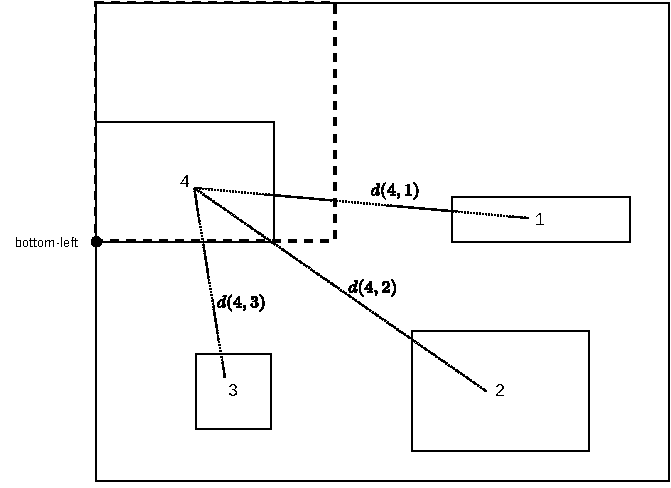
\includegraphics[width=0.8\textwidth, center]{corner_placing_heuristic}
    \caption[Painting placement example]
    {Example of a painting 4 placed inside its allocated area using the corner-placing heuristic.
    The allocated area is plotted using a dashed line.
    Also, the distances between the placed painting and all other paintings are displayed using a dotted line.}
    \label{fig:corner-placing-heuristic}
\end{figure}

\clearpage% Flush earlier floats (otherwise order might not be correct)
\newpage
\section{Operators}\label{sec:operators}
As described in section~\ref{sec:genetics}, genetic operators are used to create
new individuals.
This section presents the novel crossover and mutation genetic operators
that are used for the individual representation from section~\ref{sec:coding}.

\subsection{Crossover}\label{subsec:crossover}

Novel crossover approach proposed in this thesis
creates a new individual by weighted vector addition of the parent's stochastic vectors followed by a normalization back to the stochastic vector.
Using notation from section~\ref{sec:coding}, that is
$PS_{rk}$ for painting sequence random key vector,
$SO_{rk}$ for slicing order random key vector and
$OR_{prob}$ for orientation probabilities matrix,
we can define crossover for two parents $A$, $B$ and offspring $C$ as

\begin{equation}
    \|w_A A_{PS_{rk}} + w_B B_{PS_{rk}}\| = C_{PS_{rk}}\,,
    \label{eq:crossover-psrk}
\end{equation}

\begin{equation}
    \|w_A A_{SO_{rk}} + w_B B_{SO_{rk}}\| = C_{SO_{rk}}\,,
    \label{eq:crossover-sork}
\end{equation}

\begin{equation}
    \|P^T(w_A A_{OR_{prob}i:} + w_B B_{OR_{prob}i:})\| = C_{OR_{prob}i:}\,,
    \label{eq:crossover-orprob}
\end{equation}

where $\|\cdot\|$ is normalization to the stochastic vector\footnotemark[1], $+$ is vector addition, $w_A, w_B \in \real$ are weights,
$P \in \real^{N-1}$ is orientation penalization vector with $N$ being instance size, notation $X_{i:}$ means $i$-th row of a matrix $X$
and multiplying a vector by a scalar multiplies each element of the vector by that scalar.

\footnotetext[1]{
Normalization $\|\langle x_1, x_2, \ldots x_n \rangle\| = \langle y_1, y_2, \ldots y_n \rangle$,
    where $y_i = \dfrac{x_i}{\sum\limits_{k=1}^{n}x_k}$.
}

Example of crossover for painting sequence random key and slicing order random key (eq.~\ref{eq:crossover-psrk} and~\ref{eq:crossover-sork}),
is in figure~\ref{fig:crossover-random-keys}.
An example of crossover for orientation probabilities (eq.~\ref{eq:crossover-orprob}) is in figure~\ref{fig:crossover-orientation-probabilities}.

The crossover implementation described above has multiple parts – vector addition, weights, orientation penalization, and normalization.
Following are arguments for incorporating each of those parts into a crossover.

\subsubsection*{Vector addition and normalization}

Adding and then normalizing vectors to stochastic vectors differs from other crossover implementations.
For example, in one-point-crossover~\cite{hollandAdaptationNaturalArtificial1975} and
uniform crossover~\cite{uniformCrossover1989}, parts of the parent chromosomes are copied directly without any modification to form an offspring.

By using a stochastic vector for painting sequence random keys, slicing order random keys and rows of an orientation probability matrix,
we can interpret each of them as a probability mass function.
Next, by implementing the crossover as vector addition followed by normalization, we can
say the crossover approximates a probability mass function of some distribution from two samples, i.e., two parents.
Throughout the multiple generations, more samples are added to this approximation.
Thus, each part of the chromosome tries to approximate the probability mass function
that produces (sub)-optimal painting placement solution.

Going back to the schema theorem described subsection~\ref{subsec:schema-theorem},
we can say that the crossover proposed in this thesis does not prefer schemata with any particular order
and that length of a schema does not matter.

Preference for schemata with a short length in one-point-crossover~\cite{hollandAdaptationNaturalArtificial1975}
stems from the fact that a chromosome is split at a particular position.
This idea of splitting a chromosome is absent in the proposed approach.
For example, consider slicing order random key vector $A_{rk} = \langle 0, 0.2, 0.7, 0.1 \rangle$.
Using the decoding procedure described in~\ref{subsec:individual-decoding},
$A_{rk}$ decodes to $A = \langle 1, 4, 2, 3 \rangle$.
Then, $A$ belongs to the schema $S_1 = \langle 1, \_, \_, \_\rangle$ and also to schema $S_2 = \langle 1, \_, \_, 3 \rangle$.
$S_1$ has order 1 and $S_2$ has order 4.
Let us apply crossover to $A_{rk}$ and $B_{rk} = \langle b_1, b_2, b_3, b_4 \rangle$.
Result is $\|\langle b_1, 0.2+b_2, 0.7+b_3, 0.1+b_4 \rangle\|$.
We cannot make any assumptions about whether the result belongs to $S_1$ or $S_2$, as it purely depends on $B_{rk}$.
Additionally, we cannot predict the probability of whether $S_1$ or $S_2$ survives, i.e., they will still be present in the crossover result.
However, when using a one-point-crossover, it would depend on the position of the split.

Lastly, the proposed crossover does not prefer any particular order of schemata for the same reasons mentioned above.
It is a common feature with one-point crossover, which only prefers shorter schemata.

\subsubsection*{Weights}
Adding weights $w_A$ and $w_B$ determines the preference for transferring information from one parent to another.
The weights are calculated using a cost function $c$ from eq.~\ref{eq:objective} as

\begin{equation}
    w_A = \dfrac{c(B)}{c(A)+{c(B)}}, w_B = 1 - w_A\,.
    \label{eq:weights}
\end{equation}

Thus, the parent with better performance in the population, i.e., having lower cost function,
has more influence on what genes are being transferred to the offspring.

Adding $w_A$ and $w_B$ lowers the chance of creating offspring that do not share the advantageous schemata.
For example, considering only one stochastic vector of length three as a chromosome,
it might be advantageous to have a high value for the first value in the chromosome, e.g., $A=\langle 0.7, 0.1, 0.2 \rangle$.
On the other hand, a poorly performing individual might be $B=\langle 0.1, 0.3, 0.6 \rangle$.
Without weights, $\| A+B\| = \langle 0.4, 0.2 , 0.4 \rangle$.
Adding weights according to the eq.~\ref{eq:weights} penalizes the transfer of poorly performing schemata.

\subsubsection*{Orientation penalization}

Another part of the crossover used in the orientation probabilities matrix is the penalization vector $P$.
As mentioned in section~\ref{sec:solution-construction}, each individual decodes to one unresolved slicing tree
whose internal nodes contain a type of the cut – $H$ for horizontal, $V$ for vertical, and $*$ for a wildcard, that can take up any value $H$ or $V$.
Vector $P$ controls the preference for each type of cut.
For example, setting $P= \langle 1,1,0.5 \rangle$ penalizes only the wildcard cut $*$.
On the other hand, setting $P= \langle 1,1,1 \rangle$ removes any penalization.

The main reason for introducing $P$ is to limit the spread of wildcard cut $*$ in population,
making its appearance only at the most advantageous parts of the genes.

\begin{figure}[!htp]
    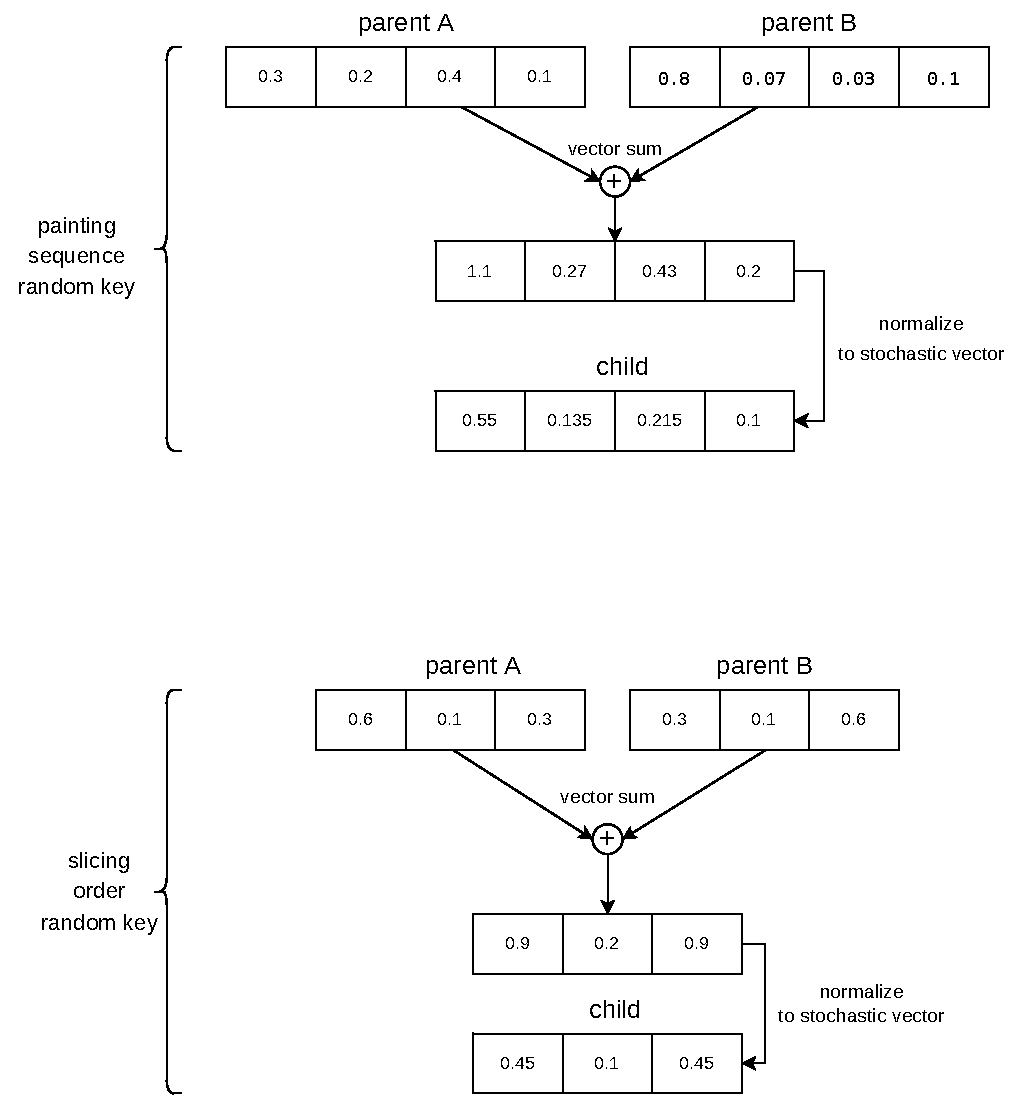
\includegraphics[width=1.0\textwidth, left]{crossover_random_keys}
    \caption[Crossover example for painting sequence and slicing order random keys]{
        Crossover example for painting sequence and slicing order random keys.
        The procedure is the same for both – sum weighted parent vectors and then normalize to stochastic vector.
    }
    \label{fig:crossover-random-keys}
\end{figure}

\begin{figure}[!htp]
    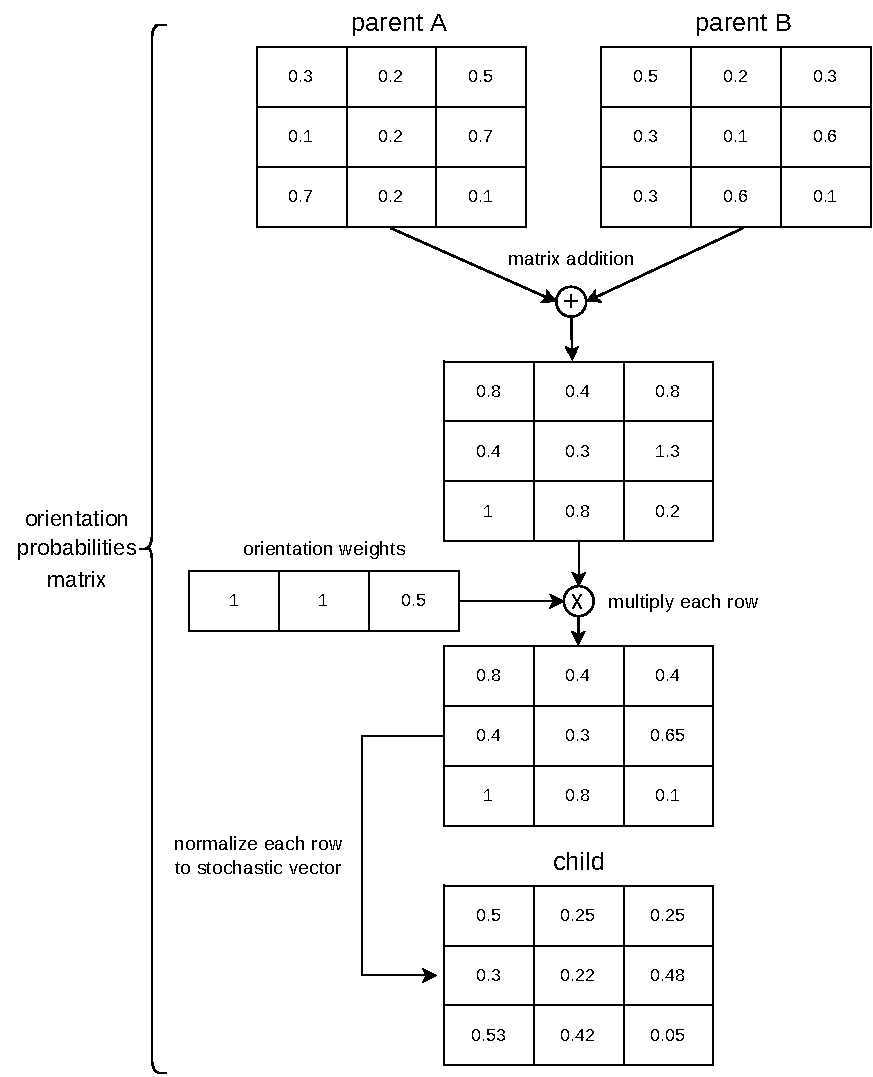
\includegraphics[width=0.85\textwidth, left]{crossover_orientation_probabilities}
    \caption[Crossover example for orientation probabilities]{
        Crossover example for orientation probabilities. The procedure is first to sum weighted parent matrices,
        then multiply the matrix with orientation penalization vector and normalize each row to a stochastic vector.}
    \label{fig:crossover-orientation-probabilities}
\end{figure}

\newpage
\subsection{Mutation}\label{subsec:mutation}

Mutation can happen on all three genes of a chromosome – painting sequence random key $PS_{rk}$,
slicing order random key $SO_{rk}$ and orientation probabilities $OR_{prob}$.
Due to the coding described in section~\ref{sec:coding}, $PS_{rk}$, $SO_{rk}$ and rows of $OR_{prob}$ are stochastic vectors.
We use this common trait and define the mutation operator for a stochastic vector as follows.

\begin{enumerate}
    \item Replace one randomly chosen element with a uniformly generated value from $\langle 0,1 \rangle$.
    \item Normalize to stochastic vector.
\end{enumerate}

With the definition of the mutation operator for a stochastic vector above, the mutation operator for an individual is defined as follows.

\begin{enumerate}
    \item Choose one of $PS_{rk}$, $SO_{rk}$, $OR_{prob}$ at random.
    \item If $PS_{rk}$ or $SO_{rk}$ is chosen, apply the mutation operator for a stochastic vector.\\
    If $OR_{prob}$ is chosen, select one row at random and apply a mutation operator for a stochastic vector.
\end{enumerate}

It is important to mention how to interpret a mutation operator.
As mentioned in section~\ref{sec:solution-construction}, an individual decodes to one unresolved slicing tree.
Mutation modifies this tree.
First, if applied to $OR_{prob}$, the value of an inner node of the tree might change.
That means a change in a type of cut – $H$, $V$, or $*$.
Second, if applied to $PS_{rk}$, the value of leaves in the tree might change.
Lastly, if applied to $SO_{rk}$, the whole structure of a tree might change.

As described above, even changing one value can result in a completely different tree and
after further decoding the slicing layout and painting placement solution.
It is the reason for defining mutation as such – to damage the chromosome as little as possible.
An example of a mutation that happens on all tree parts at once is in figure~\ref{fig:mutation}.


\begin{figure}[!h]
    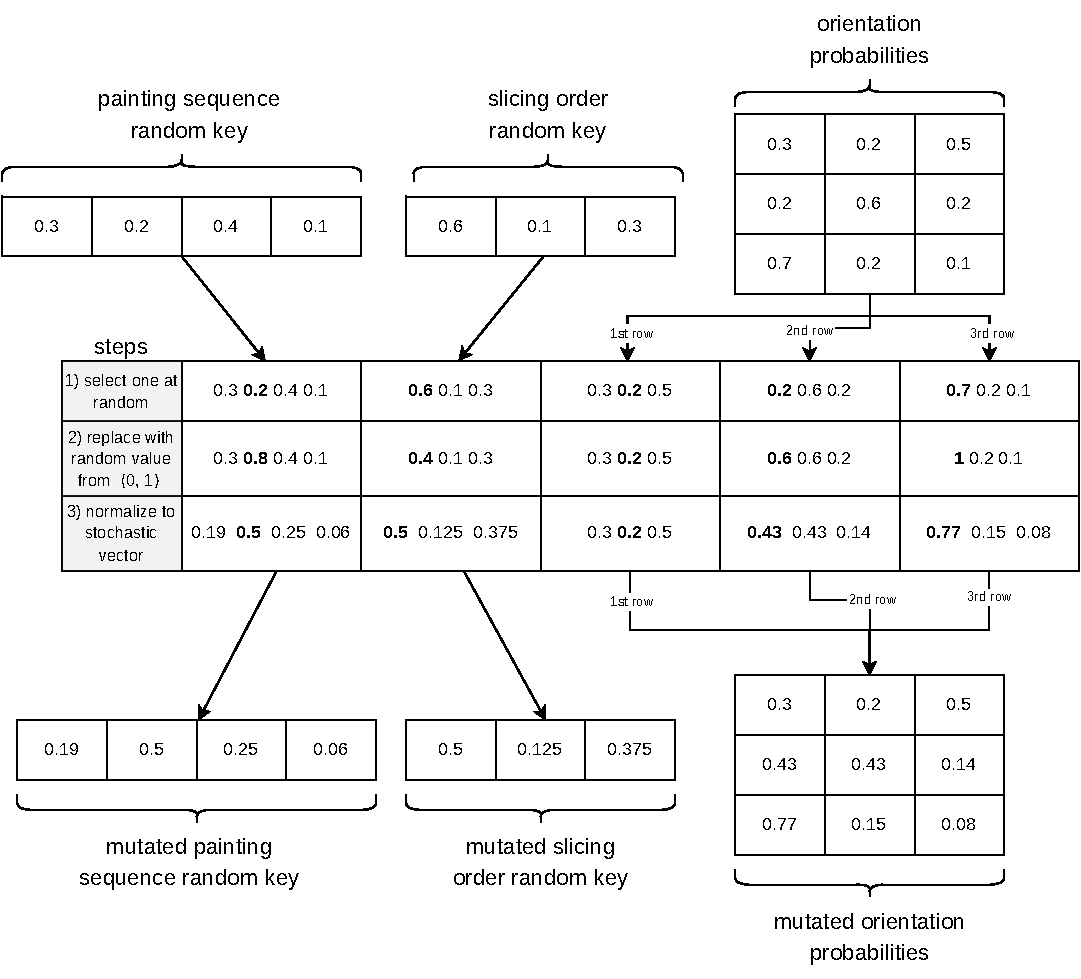
\includegraphics[width=1.0\textwidth, left]{muation}
    \caption[Example of a mutation on all three parts of a chromosome]{
        Example of a mutation on all three parts of a chromosome.
        Since all parts can be treated as a stochastic vector, the same procedure
        is used for all of them – replace one value randomly and then normalize it to a stochastic vector.
    }
    \label{fig:mutation}
\end{figure}

\clearpage% Flush earlier floats (otherwise order might not be correct)
\newpage
\section{Reproductive plan}\label{sec:reproductive-plan}

This section describes a reproductive plan used in this thesis
– a process that takes a population on input and produces a modified population using genetic operators.
The reproductive plan has two main properties that have to be well-balanced with respect to each other
– diversification and intensification~\cite{blumMetaheuristicsCombinatorialOptimization2003}.\\

\navesti{Intensification} is the ability to identify parts of the search space with a high-quality
solutions.\\

\navesti{Diversification} is the ability to prevent premature convergence to the suboptimal solutions.\\

We can classify operators in terms of their intensification and diversification effects.
The mutation operator is considered to be the most straightforward diversification strategy,
as it creates a small change in an individual's chromosome that can lead the search out of the suboptimal solution~\cite{blumMetaheuristicsCombinatorialOptimization2003}.
On the other hand, crossover creates a new solution by recombination of already present
individuals, which can be considered diversification strategy~\cite{blumMetaheuristicsCombinatorialOptimization2003}.
However, researchers in~\cite{hanshengBalanceExplorationExploitation1999} argue that crossover
also has an intensification effect. They make an argument that if the population was primarily composed of the same individuals, the crossover would not be able to improve the solution.

\subsection{Strategy}\label{subsec:strategy}
The strategy for a reproductive plan used in this thesis is in figure~\ref{fig:population-schema}.
It has two parts – generating the initial population and transitioning from one generation to the next.
After each application of the reproductive plan, the number of individuals is the same.
This means that population size is a fixed hyperparameter of the genetic approach.

\begin{figure}[!htp]
    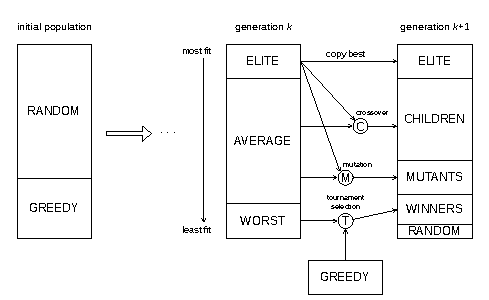
\includegraphics[width=0.8\textwidth, left]{pupulation_schema}
    \caption[Initial population generation strategy and transition]
    {Initial population generation strategy and transition from generation $k$ to $k+1$.}
    \label{fig:population-schema}
\end{figure}

\subsubsection*{Initial population}
The initial population is the population that is used as a starting point for the genetic approach.
It consists of two parts – RANDOM and GREEDY. \\

\navesti{RANDOM} part consists of randomly generated individuals.
The process of generating is (1) fill all two vectors and matrix of an individual chromosome with random values from $\langle 0,1 \rangle$
and then (2) normalize to stochastic vectors to meet constraints in~\ref{eq:constraints}.\\

\navesti{GREEDY} part consists of individuals who are, at worst, as good as RANDOM.
The process of generating $k$ GREEDY individuals is (1) to create $100k$ RANDOM individuals and (2) to select $k$ best ones
in terms of their objective value.\\

\todo{zminit duvod, proc je to zrovna takhle}

\subsubsection*{Population transition}
After generating the initial population, the genetic approach transforms the current population
to the next using crossover, mutation, selection, elitism and tournament selection.

First, the population is partitioned into three parts according to performance.\\

\navesti{ELITE} individuals are the ones that decode to the solutions with the lowest objective value.\\

\navesti{WORST} are the ones that decode to the solution the highest objective value.\\

\navesti{AVERAGE} individuals are in between the ELITE and WORST.\\

Next, the elitism strategy is used as all ELITE individuals are copied to the next generation.
Elitism enforces intensification, as it keeps the best individuals inside the population without any
modification or recombination with others.
This increases the representation of current (sub)-optimal solutions in the population, and thus it is more likely that operators increasing intensification will use ELITE as an input.
In addition, without the use of elitism, the best individual might be lost after crossing over or mutation.
\todo{pridat nejake reference do literatury}

After copying all ELITE individuals, crossover and mutation operators are used, with the crossover being
the most significant in terms of individuals that it produces for the next generation.\\

\navesti{CHILDREN} are individuals that are created using a crossover operator, with the first parent being selected
at random from ELITE and the second parent selected at random from AVERAGE.\\

\navesti{MUTANTS} are individuals that are created using a mutation operator,
with an input selected at random from ELITE and AVERAGE.\\

The two last parts of the next generation are WINNER and RANDOM.\\

\navesti{WINNER} individuals are a result of tournament selection between WORST and GREEDY.
Selection picks the best individuals from both WORST and GREEDY until all available spots for WINNER are filled. \\

The use of tournament selection between greedily generated individuals in GREEDY and the least performant
individuals in WORST is that the worst individuals are often the ones who have high penalization
values in objective~\ref{eq:objective}.
This means that they produce solutions with mostly overlapping paintings.

Lastly, a small group of randomly generated individuals RANDOM is injected into the next population.
The reason is to decrease the chance of the genetic approach getting stuck in a local optimum
by randomly adding samples from the search space.


